% Options for packages loaded elsewhere
\PassOptionsToPackage{unicode}{hyperref}
\PassOptionsToPackage{hyphens}{url}
%
\documentclass[
  english,
  man]{apa6}
\usepackage{lmodern}
\usepackage{amssymb,amsmath}
\usepackage{ifxetex,ifluatex}
\ifnum 0\ifxetex 1\fi\ifluatex 1\fi=0 % if pdftex
  \usepackage[T1]{fontenc}
  \usepackage[utf8]{inputenc}
  \usepackage{textcomp} % provide euro and other symbols
\else % if luatex or xetex
  \usepackage{unicode-math}
  \defaultfontfeatures{Scale=MatchLowercase}
  \defaultfontfeatures[\rmfamily]{Ligatures=TeX,Scale=1}
\fi
% Use upquote if available, for straight quotes in verbatim environments
\IfFileExists{upquote.sty}{\usepackage{upquote}}{}
\IfFileExists{microtype.sty}{% use microtype if available
  \usepackage[]{microtype}
  \UseMicrotypeSet[protrusion]{basicmath} % disable protrusion for tt fonts
}{}
\makeatletter
\@ifundefined{KOMAClassName}{% if non-KOMA class
  \IfFileExists{parskip.sty}{%
    \usepackage{parskip}
  }{% else
    \setlength{\parindent}{0pt}
    \setlength{\parskip}{6pt plus 2pt minus 1pt}}
}{% if KOMA class
  \KOMAoptions{parskip=half}}
\makeatother
\usepackage{xcolor}
\IfFileExists{xurl.sty}{\usepackage{xurl}}{} % add URL line breaks if available
\IfFileExists{bookmark.sty}{\usepackage{bookmark}}{\usepackage{hyperref}}
\hypersetup{
  pdftitle={The title},
  pdfauthor={First Author1 \& Ernst-August Doelle1,2},
  pdflang={en-EN},
  pdfkeywords={keywords},
  hidelinks,
  pdfcreator={LaTeX via pandoc}}
\urlstyle{same} % disable monospaced font for URLs
\usepackage{graphicx,grffile}
\makeatletter
\def\maxwidth{\ifdim\Gin@nat@width>\linewidth\linewidth\else\Gin@nat@width\fi}
\def\maxheight{\ifdim\Gin@nat@height>\textheight\textheight\else\Gin@nat@height\fi}
\makeatother
% Scale images if necessary, so that they will not overflow the page
% margins by default, and it is still possible to overwrite the defaults
% using explicit options in \includegraphics[width, height, ...]{}
\setkeys{Gin}{width=\maxwidth,height=\maxheight,keepaspectratio}
% Set default figure placement to htbp
\makeatletter
\def\fps@figure{htbp}
\makeatother
\setlength{\emergencystretch}{3em} % prevent overfull lines
\providecommand{\tightlist}{%
  \setlength{\itemsep}{0pt}\setlength{\parskip}{0pt}}
\setcounter{secnumdepth}{-\maxdimen} % remove section numbering
% Make \paragraph and \subparagraph free-standing
\ifx\paragraph\undefined\else
  \let\oldparagraph\paragraph
  \renewcommand{\paragraph}[1]{\oldparagraph{#1}\mbox{}}
\fi
\ifx\subparagraph\undefined\else
  \let\oldsubparagraph\subparagraph
  \renewcommand{\subparagraph}[1]{\oldsubparagraph{#1}\mbox{}}
\fi
% Manuscript styling
\usepackage{upgreek}
\captionsetup{font=singlespacing,justification=justified}

% Table formatting
\usepackage{longtable}
\usepackage{lscape}
% \usepackage[counterclockwise]{rotating}   % Landscape page setup for large tables
\usepackage{multirow}		% Table styling
\usepackage{tabularx}		% Control Column width
\usepackage[flushleft]{threeparttable}	% Allows for three part tables with a specified notes section
\usepackage{threeparttablex}            % Lets threeparttable work with longtable

% Create new environments so endfloat can handle them
% \newenvironment{ltable}
%   {\begin{landscape}\begin{center}\begin{threeparttable}}
%   {\end{threeparttable}\end{center}\end{landscape}}
\newenvironment{lltable}{\begin{landscape}\begin{center}\begin{ThreePartTable}}{\end{ThreePartTable}\end{center}\end{landscape}}

% Enables adjusting longtable caption width to table width
% Solution found at http://golatex.de/longtable-mit-caption-so-breit-wie-die-tabelle-t15767.html
\makeatletter
\newcommand\LastLTentrywidth{1em}
\newlength\longtablewidth
\setlength{\longtablewidth}{1in}
\newcommand{\getlongtablewidth}{\begingroup \ifcsname LT@\roman{LT@tables}\endcsname \global\longtablewidth=0pt \renewcommand{\LT@entry}[2]{\global\advance\longtablewidth by ##2\relax\gdef\LastLTentrywidth{##2}}\@nameuse{LT@\roman{LT@tables}} \fi \endgroup}

% \setlength{\parindent}{0.5in}
% \setlength{\parskip}{0pt plus 0pt minus 0pt}

% \usepackage{etoolbox}
\makeatletter
\patchcmd{\HyOrg@maketitle}
  {\section{\normalfont\normalsize\abstractname}}
  {\section*{\normalfont\normalsize\abstractname}}
  {}{\typeout{Failed to patch abstract.}}
\patchcmd{\HyOrg@maketitle}
  {\section{\protect\normalfont{\@title}}}
  {\section*{\protect\normalfont{\@title}}}
  {}{\typeout{Failed to patch title.}}
\makeatother
\shorttitle{Title}
\keywords{keywords\newline\indent Word count: X}
\DeclareDelayedFloatFlavor{ThreePartTable}{table}
\DeclareDelayedFloatFlavor{lltable}{table}
\DeclareDelayedFloatFlavor*{longtable}{table}
\makeatletter
\renewcommand{\efloat@iwrite}[1]{\immediate\expandafter\protected@write\csname efloat@post#1\endcsname{}}
\makeatother
\usepackage{lineno}

\linenumbers
\usepackage{csquotes}
\ifxetex
  % Load polyglossia as late as possible: uses bidi with RTL langages (e.g. Hebrew, Arabic)
  \usepackage{polyglossia}
  \setmainlanguage[]{english}
\else
  \usepackage[shorthands=off,main=english]{babel}
\fi

\title{The title}
\author{First Author\textsuperscript{1} \& Ernst-August Doelle\textsuperscript{1,2}}
\date{}


\authornote{

Add complete departmental affiliations for each author here. Each new line herein must be indented, like this line.

Enter author note here.

The authors made the following contributions. First Author: Conceptualization, Writing - Original Draft Preparation, Writing - Review \& Editing; Ernst-August Doelle: Writing - Review \& Editing.

Correspondence concerning this article should be addressed to First Author, Postal address. E-mail: \href{mailto:my@email.com}{\nolinkurl{my@email.com}}

}

\affiliation{\vspace{0.5cm}\textsuperscript{1} Wilhelm-Wundt-University\\\textsuperscript{2} Konstanz Business School}

\abstract{
One or two sentences providing a \textbf{basic introduction} to the field, comprehensible to a scientist in any discipline.

Two to three sentences of \textbf{more detailed background}, comprehensible to scientists in related disciplines.

One sentence clearly stating the \textbf{general problem} being addressed by this particular study.

One sentence summarizing the main result (with the words ``\textbf{here we show}'' or their equivalent).

Two or three sentences explaining what the \textbf{main result} reveals in direct comparison to what was thought to be the case previously, or how the main result adds to previous knowledge.

One or two sentences to put the results into a more \textbf{general context}.

Two or three sentences to provide a \textbf{broader perspective}, readily comprehensible to a scientist in any discipline.
}



\begin{document}
\maketitle

\hypertarget{introduction}{%
\section{Introduction}\label{introduction}}

Much recent research in third language acquisition (L3A) has been primarily concerned with the nature of cross-linguistic influence (CLI) at the initial state of L3 acquisition and has been focused on morphosyntax.
Bilinguals have, by definition, 2 linguistic systems available for transfer when they begin to learn a third language, and the precise role of these languages in L3A has been debated.
For instance, some scholars have suggested that the second language learned in late bilinguals (those who began the acquisition of the a second language (L2) after childhood) blocks access to the L1, and is the primary influence to the third language (The L2 Status Factor; Bardel and Falk (2007).
Others posit that language typology plays a decisive role in determining whether the L1 or the L2 is the primary influence on the third language (Rothman, 2010, 2011, 2013, 2015).
In this view, the individual L3 learners' subconscious impression of cross-linguistic similarity between the languages that they know in comparison to the language that they are learning determines which language primarily influences their L3.

Contrary to both the typological and L2 status views, which predict that only a single language transfers to the L3, other models suggest that cross-linguistic influence may occur on a property by property basis (Slabakova, 2017; Westergaard, Mitrofanova, Mykhaylyk, \& Rodina, 2017).
Importantly, these models have largely received support from empirical studies in morphosyntax, and thus make predictions of morphosyntactic transfer into a third language.
It is unclear whether crosslinguistic interactions of phonetics can also be predicted by the L3 morphosyntax models, since they are constrained to a larger degree in their examination of potential gradient effects in L3 learners.
For instance, two language word orders (SOV vs SVO) can directly and categorically be observed experimentally in L3 learners, in which either L1 word order or L2 word order preference is observed in a single structure of the L3.
On the other hand, and given the lack of gradience in the realization of syntactic transfer (particularly in a single observation), L3 phonetics allow for a more precise examination of the role of the L1 and the L2 to be examined in the production or perception of an acoustic signal.
For example, measurements of the acoustic realizations of L3 productions of a segment, such as voice-timing in word-initial stop consonants, may provide evidence not only for L1, L2 or property-by-property transfer, but a gradient value, which may also vary by property, and be influenced in tandem by both existing languages in the bilingual mind.
This information, together with findings in morphosyntax, can paint a clearer picture of the factors which drive CLI and how CLI interacts across phonology and morphosyntax.

The present study contributes to research on the role of the L1 and the L2 at the absolute beginning of L3 acquisition by examining the potential gradient effects of both languages on the perception of an unknown third language by Spanish-English bilinguals. Gradience in the observations allows for proportional contributions to the third language of each individual language known by a bilingual, rather that an all-or-none approach necessitated by studies in L3 morphosyntax.\\
Additionally, the present study uses four groups to experimentally control for L2 status effects and typology.
First, Spanish English bilingual participants were recruited in both orders of acquisition (English speakers who grew up monolingual and learned Spanish post-childhood and vice versa). This experimental control has not been possible in most previous studies, since the existence of these so called mirror image groups in reality is quite difficult to find and recruit. These mirror image groups have been suggested in previous studies (Puig-Mayenco, González Alonso, \& Rothman, 2020) and avoid the confound of typological transfer and L2 status (i.e.~when L2 status effects are observed, it is not simply typologically driven transfer that happens to also be the second learned language).
Secondly, the present study aims to examine how Spanish-English bilinguals categorize third language sounds by observing how they categorize two continua (a voice-timing and vowel continuum) in two different third languages, what they believe to be Hungarian (unclear relationship with Spanish and English) or French (clear Spanish-French connection).

Third, the combination of the perception of two continua in the present study, and their measurement in all three languages allows for the possibility of both gradient effects from both the L1 and the L2, a phenomenon that is much more difficult to observe in syntax, and a difference in this effect in two sound distinctions that may suggest that CLI occurs both gradiently and is structure specific.

In sum, the present study allows for the testing of four potential outcomes in the beginning stages of L3A: typological transfer, L2 transfer, structure-by-structure transfer, or gradient transfer. Unlike many previous studies, the present study controls for the teasing apart of the confound of acquisition and influence of another language by examining seemingly blank slate L3 learners. In other words, the fact that the participants in this study do not have exposure to a third language avoids the potential explanation that their results could also be caused by having acquired the structure in question, in this case language-specific voicing values for word initial stop consonants and vowels. Additionally, this use of blank-slate L3 learners allows for the recruitment of many more participants, given the scarcity of relatively homogeneous L3 learners.

\hypertarget{literature-review}{%
\section{Literature Review}\label{literature-review}}

Broadly, L3 morphosyntax models fall under two categories: full transfer models, which posit that one language is transferred to the L3 at the initial stages of L3A (also referred to as holistic transfer), and property-by-property models (The Linguistic Proximity Model, LPM; Westergaard et al., 2017, the Scalpel Model, @slabakova\_scalpel\_2017). The body of this literature review will first explain full transfer models of morphosyntax and their empirical evidence, followed property-by-property models.
Then, studies in L3 phonology will be covered in detail.
Finally, recent research in categorical perception in bilinguals will be discussed. These studies in the categorization of language specific sounds serve as the methodological basis to the present study.

\hypertarget{full-transfer-models-of-l3-morphosyntax}{%
\subsection{Full Transfer models of L3 Morphosyntax}\label{full-transfer-models-of-l3-morphosyntax}}

\hypertarget{the-typological-primacy-model}{%
\subsubsection{The Typological Primacy Model}\label{the-typological-primacy-model}}

The Typological Primacy Model (TPM; Rothman, 2013, 2010, 2011, 2015) posits that transfer of one grammar holistically occurs in the initial stages of the L3, rather than on a structure-by-structure basis.
This initial transfer is based on a subconscious \enquote{choice} or so called psycho-typology (Kellerman, 1983) made by the parser based on the cues available in the L3 input.
In particular, TPM suggests that the hierarchy for the cues used by the L3 learner to determine the typological similarity of languages (and thus which language transfers) is primarily based on cues in the L3 lexicon, followed by phonological/phonotactic information, then by functional morphology and lastly by syntactic structure.
That is, in the view of the TPM, the L3 learners will first attend to cross-linguistic similarities in the lexicon to which they are exposed via L3 input to make a determination (the L1 or the L2) of which system to transfer to the L3.
Importantly, this view of the TPM requires that the L3 learner is exposed to input.
Rothman (2015) explains that the \enquote{initial stages} of L3A are some 20-25 hours of instruction in a third language, since the L3 learner must be exposed to input before determining similarity between linguistic systems.
In the context of the present study, perceived typological proximity is predicted to be seen in distinct categorizations of what the participants believe to be French sounds as opposed to Hungarian sounds.

\hypertarget{the-l2-status-factor}{%
\subsubsection{The L2 Status Factor}\label{the-l2-status-factor}}

The L2 Status Factor (L2SF: Bardel \& Falk, 2007, 2012) posits that the second language learned serves as the source of transfer to a third language by default, regardless of typology.
Framed within the Declarative/Procedural Model (Paradis, 2004, 2009; Ullman, 2004), the L2SF suggests that the cognitive similarity of the L2 and the L3 may serve as a neurolinguistic explanation for the findings that the L2 transfers by default.
That is, within the DP model, adult L2 learners rely more heavily on declarative memory than procedural memory to learn the grammar of a new language, as opposed to L1 learning, which is learned in large part by children using procedural memory.
Since the L3 would likely also involve a higher reliance on declarative memory, it has a higher degree of similarity to the L2, which is thought to drive L2 transfer.
It is important to note that the L2 Status Factor does not make claims for simultaneous bilinguals who learn a third language later in life, or early trilinguals.
The claims made by the model refer to late bilinguals, since it is thought that they rely on declarative memory to learn a language.
However, studies involving the L2 Status Factor have found that it is possible to transfer from the L1, when L3 learners have higher metalinguistic knowledge.
Falk, Lindqvist, and Bardel (2015) examined L3 learners of a V2 language (a language that requires a verb to be the second syntactic contituent in a sentence) when their L1 was also a V2 language, and their L2 was a non-V2 language.
Using a metalinguistic awareness survey, they found that only the participants who scored higher on the survey were able to transfer their L1 V2 properties to the L3 (there was a wide range of non-V2 L2s used in the study).

\hypertarget{evidence-for-full-transfer-models}{%
\subsubsection{Evidence for full transfer models}\label{evidence-for-full-transfer-models}}

Conflicting evidence has been found in support of both of these full transfer models.
For instance, in a recent meta-analysis of 92 studies in L3 acquisition, Puig-Mayenco et al. (2020) determined that typology (59 out of 92) and L2 status (29 out of 92) were the best predictors of which linguistic system would serve as the basis for a third language.
However, these findings were not mutually exclusive; the authors coded 25 total studies as being explained both by L2 status and typology, meaning that the results of these studies reported that the L2 transferred to the L3, but could not rule out the possibility that psycho-typological transfer could also explain the results, since the studies did not use mirror image groups (i.e.~L3 groups with the same languages, but the opposite order of acquisition).
An issue with this explanation, however, is the lack of variance in the studies that the authors coded as both typological and L2 transfer, which is predicted to occur by the TPM.
If typological transfer is individually determined after exposure to L3 input (input which likely is distinct for each L3 learner), and not necessarily a reflection of actual underlying structural similarities (Rothman, 2015), then some variance would be expected to be observed in populations in which cross-linguistic typology is unclear.
In other words, one would expect that, based on the predictions of the TPM, that some learners would transfer their L1 and others would transfer their L2, particularly when there is not a clear typological similarity between the languages involved, rather than entire groups transferring solely their L1 or their L2.

Only one study has reported variance in the choice of the L1 and L2 in L3 acquisition in L3 learners whose order of acquisition was the same (i.e.~not mirror image groups seemingly driven by typology).
In the study on L3 learners of Swedish, Falk et al. (2015) found that some learners transferred their L1 and others transferred their L2 in their judgments of V2 sentences. The participants all spoke a V2 L1, and non-V2 L2, but differed in their overall metalinguistic knowledge.
The study found that participants with higher metalinguistic knowledge were able to avoid L2 status effects, which would have resulted in non-transfer from their L2, and showed facilitative transfer from L1. Although the authors suggest that this transfer is due to metalinguistic knowledge, rather than underlying perceived psychotypology, these results could also be explained by the TPM, since psycho-typological transfer is made on an individual basis.

Other studies have found that either the L1 or the L2 may transfer holistically and argue that this is evidence for holistic transfer. In a series of studies investigating the acquisition of L3 Portuguese by Spanish/English bilinguals, Rothman found that Spanish influenced L3 Portuguese, whether it was the L1 or L2 of the participants (Rothman, 2010, 2011). Other scholar report similar findings, that Spanish is the source of influence in L3 BP in Spanish-English learners of L3 BP (Parma, 2017;; Giancaspro, Halloran, \& Iverson, 2015; Cabrelli Amaro, Felipe Amaro, \& Rothman, 2015){]}, or a romance language (Italian or French) and English learning L3 Spanish Foote (2009){]}. Similarly, evidence of typologically driven influence was found from French into L3 Spanish in English-French-Spanish trilinguals (Borg, 2013; Bruhn de Garavito \& Perpiñán, 2014). It is important to mention that these studies that empirically support the TPM are exclusively combination of two romance languages (when one is the L3), and English. As a model of third language acquisition, the TPM will need to stand up cross-linguistically.

Vitally, the findings of these studies do not rule out the possibility of structure-by-structure transfer, since they typically focus on just one property per study. A dissertation that examined multiple syntactic structures in L3 French by Spanish L1 - English L2 and Turkish L1 - English L2 groups did not support the predictions of the TPM (Abbes, 2016), since the L1 Turkish group showed evidence of both L1 and L2 influence in the results. On the other hand, the Spanish L1 group showed evidence of Spanish being the sole influence on their L3 French, in line with the prediction of the TPM.

The present study engages this issue of the lack of cross-lingusitic support for the TPM by exposing 2 groups of Spanish-English (with both an English and Spanish L1) bilinguals to what they believe is French, a romance language, and what they believe is Hungarian, a non-romance language, with unclear connections to English or Spanish. Based on previous findings, the predictions of the TPM are predicted to be observed in the participants assigned to \enquote{French}, regardless of their order of acquisition (L1 English or L1 Spanish). On the other hand, it is not predicted that the TPM will be able to explain the results of the Hungarian group, where the typological relationship between the L3 and the known languages of a bilingual is ambiguous.

\hypertarget{hybrid-transfer-models-of-l3a}{%
\subsection{Hybrid Transfer models of L3A}\label{hybrid-transfer-models-of-l3a}}

\hypertarget{the-linguistic-proximity-model}{%
\subsubsection{The Linguistic Proximity Model}\label{the-linguistic-proximity-model}}

Unlike the TPM and the L2SF, the Linguistic Proximity Model (Westergaard et al., 2017) suggests that transfer occurs on a property-by-property basis, rather than holistically.
The LPM suggests that there is a \enquote{full transfer possibility}, meaning that any individual structure may transfer at any time, but that it also may not.
Scholars have argued that this vague prediction creates a problem in modeling L3 transfer acquisition (Bardel \& Falk, 2020; Wrembel, 2020), since it is unclear when transfer of a particular structure occurs and when it does not.
Likewise researchers have argued that, unlike the TPM and the L2SF, the LPM is not easily falsifiable (Bardel \& Falk, 2020).
Given the lack of predictive power of the LPM, it may only receive post-hoc support.

In the present study, it is arguable that the categorization of the L3 voice-timing continuum as one language and the categorization of the L3 vowel continuum as the other would provide support for the LPM. However, the precise reasons that a bilingual would categorize the two continua using different, language-specific perceptual boundaries would not be explained by the LPM. Unlike the TPM and L2SF, which make clear predictions, the weakness of the LPM is its unclear criteria for what triggers one language to influence L3 production and perception over the other. In the context of the present study, the LPM would be supported if participants identified the stops in the L3 continuum similarly to their L1, but identified the vowels in the L3 continuum similarly the their L2 (or vice versa). On the other hand, if each participant is found to identify both the L3 stop and vowel continua similarly to one of their two languags, then the LPM would not be supported.

\hypertarget{l3-phonology}{%
\subsection{L3 phonology}\label{l3-phonology}}

\hypertarget{studies-in-l3-phonology}{%
\subsubsection{Studies in L3 phonology}\label{studies-in-l3-phonology}}

Similar to studies in L3 morphosyntax, the few empirical studies to date in L3 phonology has endeavored to identify the source and direction of cross-linguistic influence in the linguistic sound systems of multilinguals, with particular interest in the influence of the two previously acquired systems on the third language system being acquired (Cabrelli Amaro \& Wrembel, 2016).
Various studies have found a stronger L2 influence on L3 productions at the early stages of L3 acquisition.

In a case study foundational to L3 phonology, Hammarberg and Hammarberg (1993) and Hammarberg and Hammarberg (2005) examined the productions of a single informant, who spoke L1 British English, L2 German, and L3 Swedish.
SW, a near-native German speaker as rated by German natives, was recorded reading a story in Swedish at two different time points, first one month after moving to Sweden, and second after one year having lived there.
Those Swedish recordings at both time points were then judged by native speakers of Swedish with regard to the accent of the speaker in the story, unaware that they were hearing the same informant at two different times.
Interestingly, the Swedish speakers rated the first telling of the story as heavily German accented (influence from the L2), whereas in recording 2, they rated the accent as coming from an English speaker.

This initial effect has been referred to as a \enquote{foreign language effect} (Meisel, 1983) or, more recently, as L2 status (Bardel \& Falk, 2007; Hammarberg \& Hammarberg, 2005).
The findings of Hammarberg and Hammarberg (2005) suggest that this foreign language effect, or, in other words, the desire to sound less like a speaker of one's L1, may diminish as proficiency increases and be replaced by L1 effects.
Other studies have also found primarily L2 influence in L3 productions in global accent ratings (Wrembel, 2010), VOT productions (Llama, Cardoso, \& Collins, 2010; Tremblay, 2007), vowel production (Kamiyama, 2007) vowel reduction and speech rhythm (Gut, 2010).

Other findings in L3 phonology production, however, have yielded mixed results.
Several studies have found that acoustic properties of the participants' productions fall between L1 and L3 values, suggesting that both the L1 and the L2 have some influence on L3 productions, rather than solely one language.

For instance, (Wrembel, 2014) measured VOT and aspiration in all languages of participants with two different language combinations: L1 Polish, L2 English, and L3 French; (2) L1 Polish, L2 English, and L3 German.
The results showed that each language had a specific stop-value, and that the L3 VOT productions were intermediate, falling between the L1 and L2 values.
Similarly, (Wrembel, 2011) examined thirty-two learners of L3 French with L1 Polish and L2 English who were recorded reading lists of words in carrier phrases.
As in previous studies (Wrembel, 2014), combined transfer from the L1 and the L2 in VOT productions was found.

Findings of combined L1 and L2 influence in VOT productions were also reported by Wunder (2010) in L3 Spanish speakers, and by Blank and Zimmer (2009) in L3 English speakers who spoke L1 Brazilian Portuguese and L2 French.
Other studies have found an L1 influence on production despite L3 proficiency (Wrembel, 2012), or in advanced L3 learners (Llama \& Cardoso, 2018).

Perception studies in L3 acquisition have been much more scarce than those on production, and primarily in young participants.
One of few L3 perception studies in adults is Liu, Gorba, and Cebrian (2019), which examined the perceptual boundary of a VOT continuum in trilinguals.
The participants were L3 spanish speakers who spoke L2 English and L1 Chinese.
Though the authors focused their analysis on regressive transfer and comparisons to all speakers, the reported boundaries in the study (n = 10, 28ms for Chinese, 24.6ms for English and 23ms for Spanish) suggest that the participants were using their English boundaries for L3 Spanish categorization.

Other studies in L3 perception, which have examined young trilinguals, have found a wide range of results.
For instance, Wrembel et al. (2020) found that cross-linguistic influence is structure dependent and varies among individuals, while Balas, Kopečková, and Wrembel (2019) found CLI to be modulated by a complex combination of factors such as markedness of the segment under examination, proficiency in the L2 and the L3, and L1 typology.
Finally, another study on L3 perception in young learners (Polish L1, English L2, German, L3) revealed that the L2 predominantly influences L3 perception in both rhotic sounds and devoicing of word final stops (Wrembel et al., 2020). These variable findings of the source of influence in L3 perception and production, including single langauge influence, combined languages influence, or sturcture-dependent influence, point to a lack of homogeneity in multilinguals.

Firstly, age effects in past studies have varied considerably, in both the age of onset of the L2 and the L3.
It is worth noting that many studies which report L2 status effects are in adult L3 learners, who have a late age of onset in their L2 (Hammarberg \& Hammarberg, 2005; Wrembel, 2010) or this age information was not reported (Gut, 2010; Kamiyama, 2007; Tremblay, 2007).
On the other hand, studies in which L3 learners began their acquisition of their second language at a young age (under 12) tend to show a combined effect of both the L1 and the L2 (Blank \& Zimmer, 2009; Wrembel, 2011, 2014; Wunder, 2010).
Although no study has investigated age effects and L3 transfer directly, the L2 Status Factor (Bardel \& Falk, 2007) can explain these findings based on the declarative procedural model (DP Model; Paradis, 2009, 2004; Ullman, 2004).
Based on the proposed cognitive similarities between late-learned languages in the DP model, the L2 status factor posits that the L2 will transfer to the L3 at the initial stages of acquisition.
In this view, native language grammars are known implicitly and largely subserved by the procedural memory, whereas late learned language grammars (the L2 and beyond) are thought to be more explicitly known and subserved by the declarative memory.
Importantly, the L2SF does not make predictions in regard to young bilinguals who learn a third language, precisely because the DP model would predict that both languages of young bilinguals would be implicitly known and both exist in the procedural memory.
This is in contrast to late bilinguals who learn a third language, whose native language grammar is procedural and whose L2 and L3 are declarative.

The role of proficiency in both the L2 and the L3 is another vital aspect to language transfer, and has been subject to some controversy among scholars.
In terms of proficiency in the L2, the DP model suggests that, as proficiency grows, the L2 becomes more subserved by procedural memory, and less dependent on the explicitly driven declarative memory system.
This gradual shift in dependence may result in a less clear and universal choice of language system to transfer by L2 learners in the beginning stages of L3 acquisition.
That is, it is possible that late bilinguals who are highly proficient in their L2 may pattern more like early bilinguals than late bilinguals who have lower L2 proficiency.
Other scholars argue that L2 proficiency must be sufficiently high in order for the L2 to transfer to the L3 (Rothman, 2015).
Taken together, it would seem that a threshold for L2 proficiency is necessary in order for L2 status effects to be observed.

L3 phonology studies have found conflicting evidence in the role of proficiency, and have focused on the L3, rather than L2 proficiency.
Some scholars suggest that the L2 serves as the basis for L3 transfer at low levels of L3 proficiency as a sort of \enquote{coping mechanism} (See Wrembel, 2015 for a review).
Other studies have found that L2 accented L3 speech is present in low proficiency L3 learners but that higher L3 proficiency speakers show L1 effects in their productions of their L3 (Hammarberg \& Hammarberg, 2005; Wrembel, 2010).
In sum, both L2 and L3 proficiency levels are vital and must be measured or statistically controlled to determine the precise effect of the proficiency of both languages on CLI.

Largely, with the exception of the TPM's acknowledgment of the use of phonetic cues in the input to determine cross-linguistic similarity, these models do not consider the role of phonological factors, such as language specific categorization of sounds, on cross-linguistic influence (CLI) in L3A. In principle, the predictions of these L3 morphosyntax models do not explicitly rule out their predictions of syntactic transfer as applying to phonetic CLI. A core tenet of the TPM, for instance, is the concept of cognitive economy, which suggests that one language must be holistically transferred to the L3 due to its relative cognitive ease to transferring many individual structures (Rothman, 2015). Following this argument, it is conceivably more cognitively taxing to transfer a single language's syntax and another language's phonology when a bilingual has established language specific categories in phonology and syntax in both languages than it would be to transfer the same language's syntax and phonology together. The L2 Status Factor

\hypertarget{categorical-perception}{%
\subsubsection{Categorical Perception}\label{categorical-perception}}

The present study will inform models of L3 morphosyntax by examining categorical perception of bilinguals, and determining which of the language specific categorical (phonemic) boudaries Spanish/English bilinguals use to account for L3 sounds at their first exposure.
Of the L3 morphosyntax models, only the TPM makes predictions in regard to phonological information.
Namely, it predicts that phonological or phonotactic cues are used to determine typological proximity when lexical overlap cannot readily be detected by the parser in the L3 input (Rothman, 2015).
Since the precise nature of the use of phonological information in the TPM is unclear and untested, the present study presents the same two continua to participants in order to measure their categorization of what they believe to be English, Spanish, and a third language that they do not know.

This manipulation of language mode has been carried out successfully in previous studies in both conceptual and perceptual cueing which result in language specific categorization of the same continuum.
For instance, Casillas and Simonet (2018) tested a VOT continuum of pseudowords pafri-bafri (originally used in Gonzales and Lotto (2013)) in a 2 alternative forced choice task in learners of L2 Spanish.
The stimuli differed in specific language that they were perceptually cued by a Spanish and English language-specific rhotic in the second syllable.
The results revealed that two language-specific boundaries were found in the perception of the initial stop sound in sufficiently proficient bilinguals.

In a follow up study, Lozano-Argüelles et al. (2020) also investigated Spanish English bilinguals' categorization of word initial stops /b/ and /p/.
Differently from Casillas and Simonet (2018) and Gonzales and Lotto (2013), this study presented only the first syllable of the pafri-bafri continuum (paf-baf), and manipulated the participants' language mode using conceptual cueing by telling participants they were listening to English or Spanish sounds, rather than perceptual cueing of the language specific rhotic sounds used by previous studies.
The results were consistent with previous studies; sufficiently proficient L2 Spanish speakers show language mode effects in their categorization of /p/ and /b/ on a VOT continuum, whether this is perceptually or conceptually cued.
In other words, both language-specific phonetic detail within the words were sufficient to bring about that language's categorization of the stop consonant, as well as top-down information that lead the participants to apply one of their two language-specific boundaries as a function of which language they were lead to believe that they were hearing.

\hypertarget{the-present-study}{%
\subsection{The Present Study}\label{the-present-study}}

It is this conceptual cuing that motivates the present study.
While L3 learners likely detect phonetic cross-linguistic similarities in L3 input, the present study examines the role of conceptual cueing on L3 categorization at the first exposure to L3 input.
Following the previous literature, which demonstrates that Spanish-English bilinguals categorize the same continuum of sounds differently depending upon the language they believe they are hearing, the present study both replicates these findings in the /p/-/b/ VOT continuum, extends them to a new F2 /i/-/u/ continuum, and examines whether one of these boundaries are used to categorize sounds in a new language, unknown to the speaker.
Additionally, the present study is concerned with whether the third language has a well known relationship with previously known languages, and if this affects sound categorization.

The distinction between /p/ and /b/ in Spanish is one of \enquote{true voicing}, in which a positive VOT can be observed for the \enquote{voiceless} /p/, and a positive VOT is observed in the \enquote{voiced} /b/.
English, on the other hand, has short and long lag distinction between /p/ and /b/ which is caused by a difference in aspiration.
That is, both /p/ and /b/ may be phonetically voiceless (have a positive VOT), but nevertheless be categorized as voiced and voiceless by English speakers.
French VOT varies by dialect.
Canadian French, for instance, is more similar to English in that it has the short-lag/long lag distinction, whereas European French maintains its lead/short lag distinction (Caramazza \& Yeni-Komshian, 1974).
Hungarian is considered to be a true-voicing language (Lisker \& Abramson, 1964), in which a /b/-/p/ distinction is both phonetically and phonemically voiced or voiceless.

In the case of the present study, the participants do not have any exposure to a third language, and the language-specific phonetic criteria for both voicing and vowel distinctions are of minimal importance, since the participants will not have had exposure to L3 input.
This design was chosen to inform how L3 learners will perceive input in the L3 when they engage with it for the very first time, and which of their two phonemic boundaries they will utilize.

As detailed previously, the entirety of the empirical support for the TPM comes from studies which involve two romance languages and English.
For this reason, the present study will include a group of this kind (the French L3 group), in which it is expected that the participants will account for these stimuli using their Spanish boundaries, which would partially support TPM, but provide an alternative motivation, namely top-down conceptual cueing, that is behind L3 users choice of language in situations in which typological relationship is evident.
Alternatively, an L3 Hungarian group will also be included, in which the typological relationship between the languages of this group (English, Spanish, and Hungarian) is unclear.
In this case, the categorization of what participants believe are Hungarian sounds does not have a clearly predictable pattern according to the TPM, and should result in the variable categorization of Hungarian as similar to either the L1 or the L2. Alternatively, it is possible that the Hungarian group will use their second language boundaries to categorize the L3 continua.

\hypertarget{research-questions}{%
\paragraph{Research questions}\label{research-questions}}

RQ1: Assuming that bilinguals display the same double phonemic boundary demonstrated in previous studies, which of the two language-specific phonemic boundaries will participants perceive when they are introduced to the same VOT/F2 continuum in a \enquote{third language?}
I hypothesize that that the perception of the \enquote{third language} will be modulated by the participants' order of acquisition in the event that language relatedness is unclear (the Hungarian group), and, alternatively, that participants' perception will be modulated by their knowledge about the languages relatedness when a clear connection is made between languages at an individual level (the French group).
In particular, I predict that, when hearing the same continua, participants who are led to believe they are hearing French will perceive it more closely to Spanish than English (as demonstrated by their perceptual identification of the continua).
On the other hand, I predict that participants who believe they are hearing Hungarian will categorize sounds by using the phonemic boundary of their second language (L2).
These predictions are based on findings in previous research on L3 transfer which have demonstrated the default transfer of the L2 to the L3 in language combinations which do not involve romance languages.

RQ2: Will categorizations of what participants believe to be Hungarian or French result in different \enquote{language specific} categorization?
Previous research in L3 syntactic transfer (Puig-Mayenco et al., 2020; Rothman, 2010, 2013) has suggested that language transfer to the L3 is not determined by order of acquisition, but by typological similarity of the languages involved.
The present study offers an alternative account for the data in previous studies by suggesting that the results of previous studies can be explained by a conceptual priming effect that biases the L3 learner to utilize a particular system in order to parse L3 input.
Based on findings from a systematic review of empirical studies (Puig-Mayenco et al., 2020) in L3 transfer, it appears that there is no evidence of typological transfer outside of Romance language combinations when the third language is not a Romance language.
Based on this lack of empirical support for the TPM, the present study predicts that Spanish-English bilinguals who believe that they are hearing a romance L3 will be more likely to show bias to perceive it as Spanish-like, rather than English like.
The design of the present study allows for the teasing apart of typological similarity.

\hypertarget{methods}{%
\section{Methods}\label{methods}}

\hypertarget{participants}{%
\subsection{Participants}\label{participants}}

A total of 100 participants took part in at least one experiment of the study and were recruited on the online platform Prolific. A total of 9, 1, and 6 participants did not complete all blocks of the experiment, and their data was removed from the final analysis, resulting in a total of 84 participants woh completed all portions of the experiment.
In order to tease apart L2 status effects from CLI brought about by typological similarity across languages, participants were recruited with both orders of acquisition.
That is, one group of participants spoke English as a first language and Spanish as a second language (the ES group, n = 36, and another group spoke Spanish as their first language and English as their second (the SE group, n = 55). Participants were screened prior to taking part in the study such that their age of onset was greater than 12 years old.
Then, in order to examine how the same groups of bilinguals categorize different L3s, the SE and ES group were then assigned either Hungarian (in the ES group, n = 17 and in the SE group, n =
31) or French (in the ES group, n = 17 and in the SE group, n = 18).
In order to assess whether participants were eligible to take part in the study, a screening process was carried out in prolific which involved the Language History Questionnaire ({\textbf{???}}), and a proficiency test in the participant's L2.
Speakers who reported knowing a third language or who scored below 60\% on the Lextale proficiency test were deemed ineligible for the study, and were not permitted to continue.

Low effort submissions removed: English stops 5, Spanish stops 7, 4, 1,

\hypertarget{materials}{%
\subsection{Materials}\label{materials}}

The experiment was composed of 5 total blocks
An itemized version of the Language History Questionnaire ({\textbf{???}}) was given to participants and asked their first language, second language, the age at which they began learning their L2.
The measure of L2 proficiency, the LEXTALE (Izura, Cuetos, \& Brysbaert, 2016; Lemhöfer \& Broersma, 2016), was given in Spanish to the ES group and English to the SE group.
The LEXTALE is a lexical decision task in the L2 of the participant in which the participants are presented with either a word or a non-word, and they must decide whether the word presented is a real word or a non-word.
Both the Spanish and English versions are scored in the same manner, and allow for comparability of proficiency across groups. Both versions contain 60 words total, 40 of which are real words and 20 of which are non-words. A formula then calculates a score based on the perceptage of real words correct plus the percentage of non-words correct divided by 2.

Following these tasks, participants then took a series of three two-alternative forced choice tasks (2afc).
The tasks were programmed in Psychopy (Peirce et al., 2019) and were hosted on Pavlovia.org.

\hypertarget{stimuli}{%
\subsubsection{Stimuli}\label{stimuli}}

\hypertarget{instructions}{%
\paragraph{Instructions}\label{instructions}}

Participants received written instructions prior to taking part in each phase of the experiment. The instructions for the \enquote{English} task were in English, the instructions for the \enquote{Spanish} task were in Spanish, and the instructions for the L3 tasks were bilingual (both Spanish and English). As in previous studies, the instructions contained no instances of the experimental stimuli, in this case \enquote{pafri}, \enquote{bafri,}ifri, or \enquote{ufri}, or any of their language specific forms.

\hypertarget{the-continua}{%
\paragraph{The continua}\label{the-continua}}

The 2afc tested the perception of the same two continua (a /p/-/b/ VOT continuum and a /i/-/u/ F2 continuum) in three different language modes: English, Spanish and the L3 (either Hungarian or French). The VOT continuum has been used in previous studies ((Lozano-Argüelles et al., 2020), \texttt{insert\ gonzalez\ et\ al.\ 2019\ citation\ here)} and were created from a recording by a female Spanish-English bilingual. The original VOT continuum contained the word \enquote{pafri} and \enquote{bafri}. The recording was resynthesized and ranged in VOT from -35ms to 35ms, excluding a 0 VOT step. In the present study, three additional steps were added on the positive end of the scale in order to increase the chances of /p/ responses at the positive extreme of the continuum, and made a total of 17 total steps.

The stimuli come from a female native bilingual (spanish-english) and have been used in previous studies \texttt{citations}, range from \emph{paf}-\emph{baf}.

Each continuum was created
by appending to every token on a base continuum
from baf\_ to paf\_ the ending ri portion from either a
Spanish or English pronunciation of pafri (Spanish /ri/ or
English /ai/), as appropriate."

During the 2afc task, participants saw both the words \emph{pafri} and \emph{bafri} on the screen (also used in \texttt{citation}), and hear just the first syllable of these words in which the initial consonant was a member of the continuum.
Each step of the continuum was played 5 times total, leading to a total of 85 trials in the VOT continuum per participant. Each trial was drawn randomly from the continuum in a single block, so no participant heard the same stimulus order.
The F2 continuum followed the same procedure, but contained 11 steps in an F2 continuum ranging from X to X hertz.
Due to language spefific differences in vowel space, the non-words on screen were distinct orthographically in each language, with the exception of French and Spanish.
In Spanish and French, the participants saw \emph{ifri} and \emph{ufri} on the screen, in English they say \emph{eefri} and \emph{oofri}, and in Hungarian, they say \emph{ifrelo} and \emph{ufrelo}.
All participants heard one member of the same /if/-/uf/ continuum across all trails.
The stimuli for the vowel continuum were created in PRAAT (Boersma \& Weenink, 2021) and were originally produced by a male speaker of American English.
The original sounds were re-synthesized to create a continuum using a PRAAT script (Boersma \& Weenink, 2021).

\hypertarget{procedure}{%
\subsection{Procedure}\label{procedure}}

All participants completed a total of five tasks, the Language History Questionnaire, the LEXTALE proficiency test in their L2, and three two alternative forced choice tasks. First, the participants completed the Language History Questionnaire online ({\textbf{???}}), followed by the LEXTALE proficiency test.
Following these two tasks used for screening, only those participants who did have knowledge of a third language and scored at least 60\% on the LEXTALE were deemed eligible and continued the experiment.
Following these screening tasks, and in order to control for language mode, the participants completed the 2afc tasks in a semi-longitudinal design.
Participants were invited to take part in the second portion of the experiment at least 30 minutes after their completion of the previous step.
All participants began with the \enquote{English} task, followed by \enquote{Spanish}, and finished with either \enquote{French} or \enquote{Hungarian}.
In the English and Spanish tasks, the instructions were given in that respective language, and it was explained that the participants were going to hear rare words in the language in question (English, Spanish or the L3).
In the L3 session, the same instructions were given in both English and Spanish in order to avoid biasing the participants to either English or Spanish mode.

\hypertarget{statistical-analyses}{%
\subsection{Statistical analyses}\label{statistical-analyses}}

In order to determine a crossover boundary for analysis in a general linear model, two logistic regression models were fit to each participant with their responses of \enquote{bafri}/\enquote{pafri}, in the VOT continuum, and \enquote{ifri/ufri}, in the F2 continuum as a function of the standardized continuum step for each language. The continuum step standardization was done in order to allow for the comparabiltiy of the L1 and L2 crossover boundaries, which had a distinct number of steps. As a result, 6 crossover boundaries total were calculated per participant that provided which step in the continuum the probability of the participant choosing either \enquote{pafri} or \enquote{bafri} was 50\%. These boundaries were used as continuous variables in subsequent general linear regression models and t.tests. All analyses were carried out in R ({\textbf{???}}) and used either the stats package or the lmer package ({\textbf{???}}).

In order to determine the independence of the crossover samples, paired t.tests were carried out in each language combinaton in both stops and vowels. A significant p-value on a paired t-test would indicate that there is non-zero difference between individual participants' crossover boundaries between two languages on average. Based on the results of the paired t-tests, 2 general linear models (GLMs) were run for the Spanish L1 group, but not the English L1 group, since the paired t-tests in the English group did not reveal a double phonetmic boundary effect in either stops (\(t(26) = -0.98\), \(p = .338\)), or vowels (\(t(35) = -0.72\), \(p = .477\)). The two GLMs that were run predicted the L3 crossover boundary in vowels (in the first model) and in stops (in the second model). The independent variables included the continuous predictors L1 crossover boundary(L1 co), L2 crossover boundary (L2 co) and the categorical variable L3 group (French or Hungarian). The best fitting model, as well as main effects and interactions, were derived from nested model comparisons using the anova function and model assumptions were tested with the gvlma function in R (({\textbf{???}})). P-values are reported with alpha set at .05.

\hypertarget{results}{%
\section{Results}\label{results}}

\hypertarget{vowels}{%
\subsection{Vowels}\label{vowels}}

Figure 1 shows the categorizations of the vowel continuum by both L1 groups in English and Spanish. A series of paired t-tests were used to determine whether the participant groups categorized the continua differently as a function of the language that they were lead to believe that they were hearing.
A paired t-test revealed that Spanish and English were categorized differently in the Spanish L1 group for vowels (\(t(50) = -2.77\), \(p = .008\)), implying a double phonemic boundary effect. However, this effect was not detected between the categorization of the vowel continuum in the English group \(t(35) = -0.72\), \(p = .477\)).

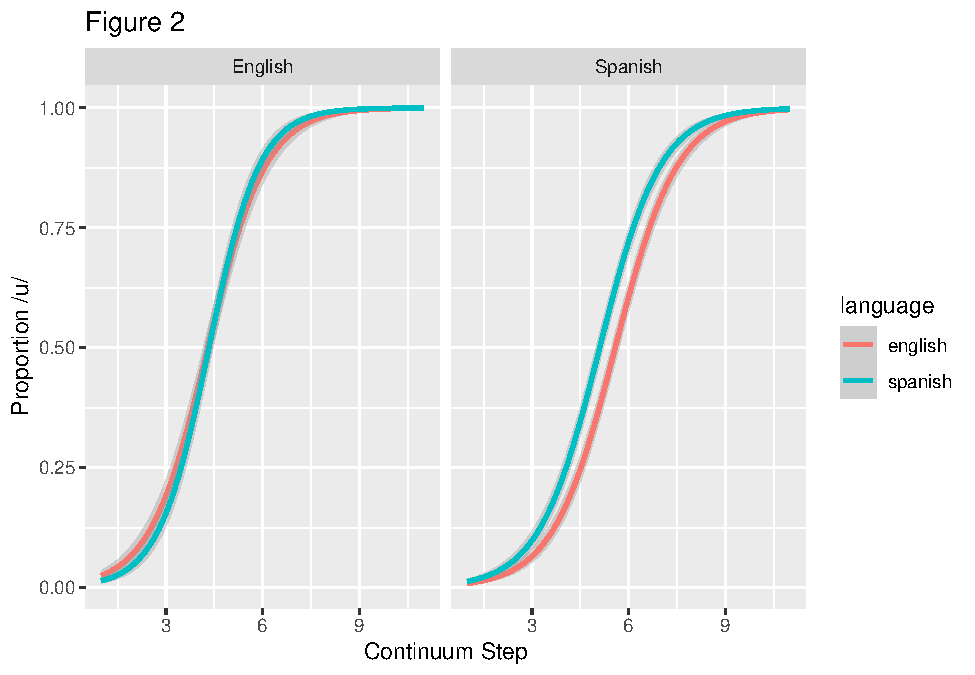
\includegraphics{master_files/figure-latex/unnamed-chunk-1-1.pdf}

Since only the Spanish L1 group showed this double phonemic boundary effect in vowels, this was the only group that could truly inform whether Spanish-English bilinguals categorize L3 sounds according to their L1 or L2 perceptual routines. In other words, since the English L1 group did not categorize the Spanish and English continua as differently, it cannot be determined whether their Spanish or English has a greater impact on their L3 perception. As a result, the following analysis will focus on the vowel categorizations of the Spanish L1 group.

Figure 2 shows the categorizations of the L1 Spanish group by L3 group. Paired t-tests revealed that L2 (English) was categorized differently from the L3 in both the French L3 group (\(t(16) = 3.20\), \(p = .006\)) and the Hungarian L3 group (\(t(28) = 2.46\), \(p = .020\)). Similarly, another set of paired t-tests revealed that both of these groups did not categorize their L1 (Spanish) as differently from Hungarian (\(t(28) = -0.82\), \(p = .418\)) or French (\(t(16) = -0.91\), \(p = .376\)). A t-test comparing the categorizations between the two L1 Spanish L3 groups suggested that the these categorizations were also not distinct (\(t(30.53) = 0.14\), \(p = .893\)).

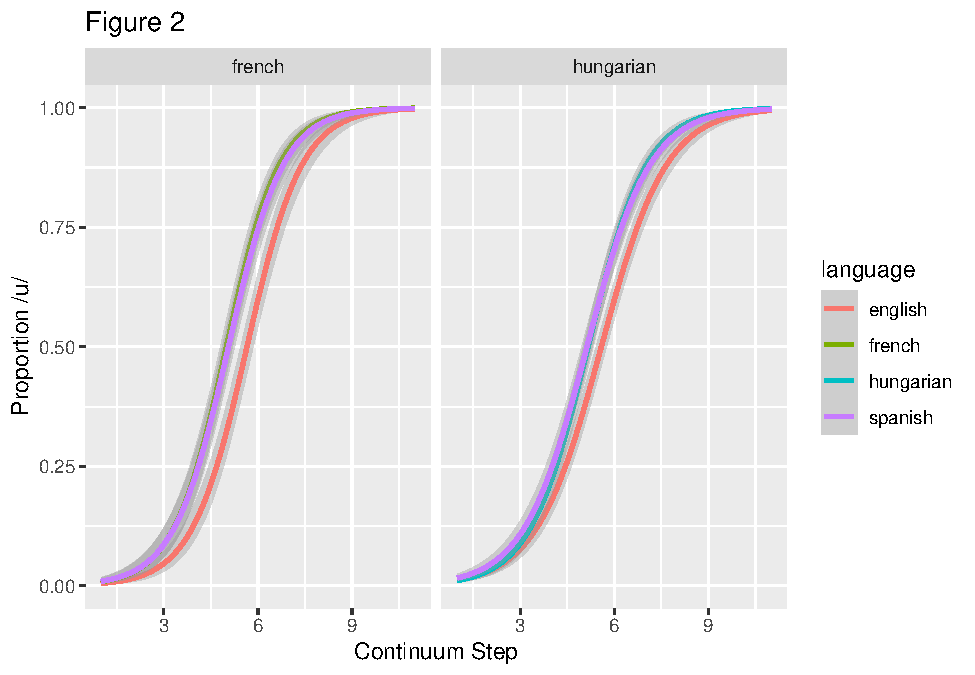
\includegraphics{master_files/figure-latex/unnamed-chunk-2-1.pdf}

The Spanish L1 group (\(t(53) = -1.10\), \(p = .278\)).

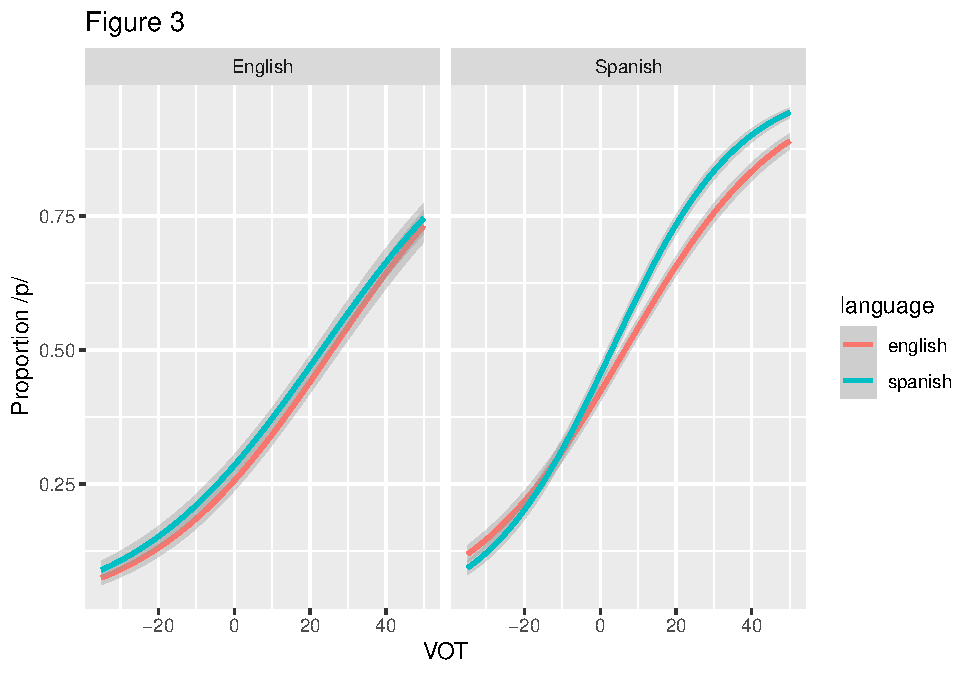
\includegraphics{master_files/figure-latex/unnamed-chunk-3-1.pdf}

Table 1 shows the cross-over boundaries of each group in each language.

\begin{table}[tbp]

\begin{center}
\begin{threeparttable}

\caption{\label{tab:unnamed-chunk-4}Descriptive statistics of vowel crossovers by group}

\begin{tabular}{llllll}
\toprule
l1 & \multicolumn{1}{c}{l3\_group} & \multicolumn{1}{c}{mean\_english} & \multicolumn{1}{c}{mean\_spanish} & \multicolumn{1}{c}{mean\_l3} & \multicolumn{1}{c}{n}\\
\midrule
English & french & -0.14 & -0.13 & -0.14 & 17\\
English & hungarian & -0.14 & -0.13 & -0.13 & 17\\
Spanish & french & -0.07 & -0.11 & -0.10 & 17\\
Spanish & hungarian & -0.08 & -0.11 & -0.10 & 29\\
\bottomrule
\end{tabular}

\end{threeparttable}
\end{center}

\end{table}

\begin{table}[tbp]

\begin{center}
\begin{threeparttable}

\caption{\label{tab:unnamed-chunk-5}Descriptive statistics of stop crossovers by group}

\begin{tabular}{llllll}
\toprule
l1 & \multicolumn{1}{c}{l3\_group} & \multicolumn{1}{c}{mean\_english} & \multicolumn{1}{c}{mean\_spanish} & \multicolumn{1}{c}{mean\_l3} & \multicolumn{1}{c}{n}\\
\midrule
English & french & 0.51 & 0.51 & 0.60 & 11\\
English & hungarian & 0.51 & 0.51 & 0.20 & 14\\
Spanish & french & -0.17 & -0.17 & -0.33 & 18\\
Spanish & hungarian & -0.03 & -0.03 & -0.13 & 30\\
\bottomrule
\end{tabular}

\end{threeparttable}
\end{center}

\end{table}

\begin{table}[tbp]

\begin{center}
\begin{threeparttable}

\caption{\label{tab:unnamed-chunk-6}A regression table.}

\begin{tabular}{lllll}
\toprule
Predictor & \multicolumn{1}{c}{$b$} & \multicolumn{1}{c}{95\% CI} & \multicolumn{1}{c}{$t(41)$} & \multicolumn{1}{c}{$p$}\\
\midrule
Intercept & -0.04 & $[-0.06$, $-0.02]$ & -3.44 & .001\\
L1 & 0.28 & $[0.16$, $0.41]$ & 4.67 & < .001\\
L2 & 0.15 & $[-0.18$, $0.48]$ & 0.91 & .369\\
L3 grouphungarian & 0.00 & $[-0.02$, $0.02]$ & -0.13 & .900\\
L1 $\times$ L2 & -2.03 & $[-3.65$, $-0.41]$ & -2.53 & .015\\
\bottomrule
\end{tabular}

\end{threeparttable}
\end{center}

\end{table}

\hypertarget{discussion}{%
\section{Discussion}\label{discussion}}

\hypertarget{general-discussion}{%
\subsection{General Discussion}\label{general-discussion}}

The present study attempted to replicate the double phonemic boundary effect in adult Spanish-English bilinguals in both orders of acquisition in two continua, a voicing continuum, and a vowel continuum, in order to investigate how laguage specific categorization of the continua interacted with a third language at first exposure that the participants did not know, either French or Hungarian. Vitally, language activation was conceptually cued the sounds on each step of both continua were acoustically identical. The 2 alternative forced choice tasks only differed in the language of the instructions (Spanish for the Spanish session, English for the English session, and bilingual for the L3 session), and the spellings of the stimuli. These tasks both attempt to replicate the findings of a double phonemic boundary effect found in previous studies \texttt{citations}, and to examine whether a double phonemic boundary is present in vowels. The results revealed that, unlike previous studies, that the participants in the English L1 group did not show a double phonemic boundary effect in the voicing continuum, since no reliable difference was found in their categorization of the VOT continuum across experiments. The English L1 group also did not show a double phonemic boundary effect in vowels. The Spanish L1 group, on the other hand, did display language specific categorizations of /i/ and /u/ in their L1 and their L2, but not in the stop continuum. As a result, the data of the L3 continua categorizations could only be examined in the Spanish L1 group with vowels, since this was the only case where participants treated their L1 and L2 differently. The data revealed that both the Hungarian and French groups categorized what they believed to be their L3 as similar to Spanish, their L1.

\hypertarget{revisiting-the-predictions-of-l3-models}{%
\subsection{Revisiting the predictions of L3 models}\label{revisiting-the-predictions-of-l3-models}}

None of the predictions of the Typological Primacy Model, the L2 Status Factor, or the Linguistic Proximity Model were supported by these results.The TPM would have predicted that the French L3 groups would categorize both French continua as similar to their individual Spanish continua, whether they spoke Spanish as their L1 or English. The TPM's predictions for the Hungarian groups, on the other hand, are not quite as clear. The TPM posits that, on an individual basis, one entire language is the primary influence on the L3, and that this determination is made on the basis of exposure to input. Previous findings that support the TPM include language combinations that include 2 romance language and English, and no variability in the individual's \enquote{choice} of transfer has been reported. This lack of variability has been explained by Rothman as having been due to the \enquote{obvious} proximity of two romance languages relative to English. This explanation may hold water in that L3 learners are metalinguistically guided in their processing of an L3 at the early stages of acquisition in the event that they speak a romance language and English and are learning a third language that is also a romance language. However, this logic does not lead to clear predictions when the third language has an ambiguous relationship with the L1 and the L2. In the case of Spanish, English and Hungarian, it's rather unclear what \enquote{obvious} connections exist between any two of the three languages. In this case, the TPM might predict variability in the choice of holistic transfer; that some participants will be influenced by their L1 or by their L2 when they are exposed to a third language, but that both will exist in both orders of acquisition. However, the TPM does not make clear predictions as to which participants will choose their L1 and which will choose their L2, not whether one will be more common.

Additionally, the claim of the TPM that cognitive economy brings about whole language cross-linguistic influence does not hold up here: the Spanish L1 group categorized the L3 continua similarly to their L1 with vowels, but did not do so for stops. These results suggest that, firstly, there is a gradient effect of influence from both language systems, and, secondly, that this effect may vary by phoneme. A potential limitation of examining cross linguistic influence via the study of morphosyntax is that the two specific syntaxes offer the speaker a binary choice in many cases. As a result, models of morphosyntax should not make claims or predictions regarding CLI in a non-gradient and categorical manner. It would seem that the influence of both languages on the L3 is both gradient and structure dependent, and given the variability between groups and lack of explanatory power of proficiency, it may also be a dynamic, ever-changing relationship, in line with the tenets of Dynamic Systems Theory (DST, \texttt{citation}). Some scholars have applied DST to multilingualism \texttt{Jessner\ and\ friend\ citation} and argue that the language systems of a multilingual are ever changing and deferentially intertwined throughout time. This view of langauges as dynamic, non-static systems complicates the idea of predictive modeling since it is more difficult to find many multilingual speakers that are alike in the many factors that influence the interplay of language systems such as language use, proficiency, and age effects.

The L2SF predicted a default influence of the L2 on the L3.

These results do not mirror results in L3 phonology studies on production, nor the few studies in perception.

These results also failed to replicate the results of previous studies in categorical perception in the English L1 group for both stops and vowels, but found a double phonemic boundary effect for the vowel continuum in the Spanish L1 group. It is unclear why\ldots. post-hoc proficiency stats\ldots{}

\hypertarget{references}{%
\section{References}\label{references}}

\begingroup
\setlength{\parindent}{-0.5in}
\setlength{\leftskip}{0.5in}

\hypertarget{refs}{}
\leavevmode\hypertarget{ref-abbes_acquisition_2016}{}%
Abbes, K. B. (2016). The acquisition of french morpho-syntactic properties: Cross-linguistic influence in the learning of l3 french by turkish/spanish speakers who learned english as an l2. \url{https://doi.org/10.13140/RG.2.2.35972.78726}

\leavevmode\hypertarget{ref-balas_perception_2019}{}%
Balas, A., Kopečková, R., \& Wrembel, M. (2019). PERCEPTION OF RHOTICS BY MULTILINGUAL CHILDREN. In S. Calhoun, P. Escudero, M. Tabain, \& P. Warren (Eds.), \emph{Proceedings of the 19th international congress of phonetic sciences}. Melbourne, Australia: Canberra, Australia: Australasian Speech Science; Technology Association Inc.

\leavevmode\hypertarget{ref-bardel_role_2007}{}%
Bardel, C., \& Falk, Y. (2007). The role of the second language in third language acquisition: The case of germanic syntax. \emph{Second Language Research}, \emph{23}(4), 459--484. \url{https://doi.org/10.1177/0267658307080557}

\leavevmode\hypertarget{ref-cabrelli_amaro_l2_2012}{}%
Bardel, C., \& Falk, Y. (2012). The l2 status factor and the declarative/procedural distinction. In J. Cabrelli Amaro, S. Flynn, \& J. Rothman (Eds.), \emph{Studies in bilingualism} (Vol. 46, pp. 61--78). Amsterdam: John Benjamins Publishing Company. \url{https://doi.org/10.1075/sibil.46.06bar}

\leavevmode\hypertarget{ref-bardel_l1_2020}{}%
Bardel, C., \& Falk, Y. (2020). L1, l2 and l3: Same or different? \emph{Second Language Research}, 026765832094103. \url{https://doi.org/10.1177/0267658320941033}

\leavevmode\hypertarget{ref-blank_transferencia_2009}{}%
Blank, C. A., \& Zimmer, M. C. (2009). A transferência fonético-fonológica l2 (francês) -- l3 (inglês): Um estudo de caso. \emph{Revista de Estudos Da Linguagem}, \emph{17}(1), 207--233. \url{https://doi.org/10.17851/2237-2083.17.1.207-233}

\leavevmode\hypertarget{ref-borg_acquisition_2013}{}%
Borg, K. (2013). The acquisition of future of probability in l3 spanish. In \emph{Proceedings of the 12th generative approaches to second language acquisition}. Sommervilla, MA: Cascadilla Proceedings Project.

\leavevmode\hypertarget{ref-bruhn_de_garavito_subject_2014}{}%
Bruhn de Garavito, J., \& Perpiñán, S. (2014). Subject pronouns and clitics in the spanish interlanguage of french l1 speakers. In \emph{Subject pronouns and clitics in the spanish interlanguage of french l1 speakers}.

\leavevmode\hypertarget{ref-peukert_relationship_2015}{}%
Cabrelli Amaro, J., Felipe Amaro, J., \& Rothman, J. (2015). The relationship between l3 transfer and structural similarity across development: Raising across an experiencer in brazilian portuguese. In H. Peukert (Ed.), \emph{Hamburg studies on linguistic diversity} (Vol. 4, pp. 21--52). Amsterdam: John Benjamins Publishing Company. \url{https://doi.org/10.1075/hsld.4.02ama}

\leavevmode\hypertarget{ref-cabrelli_amaro_investigating_2016}{}%
Cabrelli Amaro, J., \& Wrembel, M. (2016). Investigating the acquisition of phonology in a third language -- a state of the science and an outlook for the future. \emph{International Journal of Multilingualism}, \emph{13}(4), 395--409. \url{https://doi.org/10.1080/14790718.2016.1217601}

\leavevmode\hypertarget{ref-caramazza_voice_1974}{}%
Caramazza, A., \& Yeni-Komshian, G. H. (1974). Voice onset time in two french dialects. \emph{Journal of Phonetics}, \emph{2}(3), 239--245. \url{https://doi.org/10.1016/S0095-4470(19)31274-4}

\leavevmode\hypertarget{ref-casillas_perceptual_2018}{}%
Casillas, J. V., \& Simonet, M. (2018). Perceptual categorization and bilingual language modes: Assessing the double phonemic boundary in early and late bilinguals. \emph{Journal of Phonetics}, \emph{71}, 51--64. \url{https://doi.org/10.1016/j.wocn.2018.07.002}

\leavevmode\hypertarget{ref-falk_role_2015}{}%
Falk, Y., Lindqvist, C., \& Bardel, C. (2015). The role of l1 explicit metalinguistic knowledge in l3 oral production at the initial state. \emph{Bilingualism: Language and Cognition}, \emph{18}(2), 227--235. \url{https://doi.org/10.1017/S1366728913000552}

\leavevmode\hypertarget{ref-foote_transfer_2009}{}%
Foote, R. (2009). Transfer in l3 acquisition: The role of typology. In Y.-k. I. Leung (Ed.), \emph{Third language acquisition and universal grammar}. Bristol, UK ; Buffalo, NY: Multilingual Matters.

\leavevmode\hypertarget{ref-giancaspro_transfer_2015}{}%
Giancaspro, D., Halloran, B., \& Iverson, M. (2015). Transfer at the initial stages of l3 brazilian portuguese: A look at three groups of english/spanish bilinguals. \emph{Bilingualism: Language and Cognition}, \emph{18}(2), 191--207. \url{https://doi.org/10.1017/S1366728914000339}

\leavevmode\hypertarget{ref-gonzales_bafri_2013}{}%
Gonzales, K., \& Lotto, A. J. (2013). A \emph{bafri} , un \emph{pafri}: Bilinguals' pseudoword identifications support language-specific phonetic systems. \emph{Psychological Science}, \emph{24}(11), 2135--2142. \url{https://doi.org/10.1177/0956797613486485}

\leavevmode\hypertarget{ref-gut_cross-linguistic_2010}{}%
Gut, U. (2010). Cross-linguistic influence in l3 phonological acquisition. \emph{International Journal of Multilingualism}, \emph{7}(1), 19--38. \url{https://doi.org/10.1080/14790710902972248}

\leavevmode\hypertarget{ref-hammarberg_articulatory_1993}{}%
Hammarberg, B., \& Hammarberg, B. (1993). Articulatory re-setting in the acquisition of new languages. \emph{Phonum}, \emph{2}, 61--67.

\leavevmode\hypertarget{ref-hammarberg_processes_2005}{}%
Hammarberg, B., \& Hammarberg, B. (2005). \emph{Processes in third language acquisition}. Edinburgh University Press. \url{https://doi.org/10.3366/edinburgh/9780748635115.001.0001}

\leavevmode\hypertarget{ref-izura_lexical_2016}{}%
Izura, C., Cuetos, F., \& Brysbaert, M. (2016). \emph{Lexical test for advanced learners of spanish}. American Psychological Association. \url{https://doi.org/10.1037/t47086-000}

\leavevmode\hypertarget{ref-kamiyama_acquisition_2007}{}%
Kamiyama, T. (2007). Acquisition of french vowels by japanese-speaking learners: Close and close-mid rounded vowels. In \emph{Acquisition of french vowels by japanese-speaking learners: Close and close-mid rounded vowels}. Freiburg, Germany.

\leavevmode\hypertarget{ref-kellerman_now_1983}{}%
Kellerman, E. (1983). Now you see it, now you don't. In \emph{Language transfer in language learning} (pp. 112--134). Rowley, MA: Newbury House.

\leavevmode\hypertarget{ref-lemhofer_lexical_2016}{}%
Lemhöfer, K., \& Broersma, M. (2016). \emph{Lexical test for advanced learners of english}. American Psychological Association. \url{https://doi.org/10.1037/t47085-000}

\leavevmode\hypertarget{ref-lisker_cross-language_1964}{}%
Lisker, L., \& Abramson, A. S. (1964). A cross-language study of voicing in initial stops: Acoustical measurements. \emph{\textup{WORD}}, \emph{20}(3), 384--422. \url{https://doi.org/10.1080/00437956.1964.11659830}

\leavevmode\hypertarget{ref-liu_effects_2019}{}%
Liu, Z., Gorba, C., \& Cebrian, J. (2019). EFFECTS OF LEARNING AN ADDITIONAL LANGUAGE ON VOT PERCEPTION. In S. Calhoun, P. Escudero, M. Tabain, \& P. Warren (Eds.), \emph{Proceedings of the 19th international congress of phonetic sciences} (pp. 3750--3753). Melbourne, Australia: Canberra, Australia: Australasian Speech Science; Technology Association Inc.

\leavevmode\hypertarget{ref-llama_revisiting_2018}{}%
Llama, R., \& Cardoso, W. (2018). Revisiting (non-)native influence in VOT production: Insights from advanced l3 spanish. \emph{Languages}, \emph{3}(3), 30. \url{https://doi.org/10.3390/languages3030030}

\leavevmode\hypertarget{ref-llama_influence_2010}{}%
Llama, R., Cardoso, W., \& Collins, L. (2010). The influence of language distance and language status on the acquisition of l3 phonology. \emph{International Journal of Multilingualism}, \emph{7}(1), 39--57. \url{https://doi.org/10.1080/14790710902972255}

\leavevmode\hypertarget{ref-lozano-arguelles_conceptually_2020}{}%
Lozano-Argüelles, C., Fernández Arroyo, L., Rodríguez, N., Durand López, E. M., Garrido Pozú, J. J., Markovits, J., \ldots{} Casillas, J. V. (2020). CONCEPTUALLY CUED PERCEPTUAL CATEGORIZATION IN ADULT l2 LEARNERS. \emph{Studies in Second Language Acquisition}, 1--16. \url{https://doi.org/10.1017/S0272263120000273}

\leavevmode\hypertarget{ref-meisel_transfer_1983}{}%
Meisel, J. M. (1983). Transfer as a second-language strategy. \emph{Language \& Communication}, \emph{3}(1), 11--46. \url{https://doi.org/10.1016/0271-5309(83)90018-6}

\leavevmode\hypertarget{ref-paradis_neurolinguistic_2004}{}%
Paradis, M. (2004). \emph{A neurolinguistic theory of bilingualism}. Amsterdam ; Philadelphia: J. Benjamins Pub.

\leavevmode\hypertarget{ref-paradis_declarative_2009}{}%
Paradis, M. (2009). \emph{Declarative and procedural determinants of second languages} (Vol. 40). Amsterdam: John Benjamins Publishing Company. \url{https://doi.org/10.1075/sibil.40}

\leavevmode\hypertarget{ref-parma_cross-linguistic_2017}{}%
Parma, A. (2017). Cross-linguistic transfer of object clitic structure: A case of l3 brazilian portuguese. \emph{Languages}, \emph{2}(3), 14. \url{https://doi.org/10.3390/languages2030014}

\leavevmode\hypertarget{ref-peirce_psychopy2_2019}{}%
Peirce, J., Gray, J. R., Simpson, S., MacAskill, M., Höchenberger, R., Sogo, H., \ldots{} Lindeløv, J. K. (2019). PsychoPy2: Experiments in behavior made easy. \emph{Behavior Research Methods}, \emph{51}(1), 195--203. \url{https://doi.org/10.3758/s13428-018-01193-y}

\leavevmode\hypertarget{ref-puig-mayenco_systematic_2020}{}%
Puig-Mayenco, E., González Alonso, J., \& Rothman, J. (2020). A systematic review of transfer studies in third language acquisition. \emph{Second Language Research}, \emph{36}(1), 31--64. \url{https://doi.org/10.1177/0267658318809147}

\leavevmode\hypertarget{ref-rothman_typological_2010}{}%
Rothman, J. (2010). On the typological economy of syntactic transfer: Word order and relative clause high/low attachment preference in l3 brazilian portuguese. \emph{IRAL - International Review of Applied Linguistics in Language Teaching}, \emph{48}(2). \url{https://doi.org/10.1515/iral.2010.011}

\leavevmode\hypertarget{ref-rothman_l3_2011}{}%
Rothman, J. (2011). L3 syntactic transfer selectivity and typological determinacy: The typological primacy model. \emph{Second Language Research}, \emph{27}(1), 107--127. \url{https://doi.org/10.1177/0267658310386439}

\leavevmode\hypertarget{ref-baauw_cognitive_2013}{}%
Rothman, J. (2013). Cognitive economy, non-redundancy and typological primacy in l3 acquisition: Initial stages of l3 romance and beyond. In S. Baauw, F. Drijkoningen, L. Meroni, \& M. Pinto (Eds.), \emph{Romance languages and linguistic theory} (Vol. 5, pp. 217--248). Amsterdam: John Benjamins Publishing Company. \url{https://doi.org/10.1075/rllt.5.11rot}

\leavevmode\hypertarget{ref-rothman_linguistic_2015}{}%
Rothman, J. (2015). Linguistic and cognitive motivations for the typological primacy model (TPM) of third language (l3) transfer: Timing of acquisition and proficiency considered. \emph{Bilingualism: Language and Cognition}, \emph{18}(2), 179--190. \url{https://doi.org/10.1017/S136672891300059X}

\leavevmode\hypertarget{ref-slabakova_scalpel_2017}{}%
Slabakova, R. (2017). The scalpel model of third language acquisition. \emph{International Journal of Bilingualism}, \emph{21}(6), 651--665. \url{https://doi.org/10.1177/1367006916655413}

\leavevmode\hypertarget{ref-tremblay_l2_2007}{}%
Tremblay, M. (2007). L2 influence on l3 pronunciation: Native-like VOT in the l3 japanese of english-french bilinguals. In. Presented at the Papers presented at the l3 phonology satellite workshop of ICPhS XVI, Freiburg, Germany.

\leavevmode\hypertarget{ref-ullman_contributions_2004}{}%
Ullman, M. T. (2004). Contributions of memory circuits to language: The declarative/procedural model. \emph{Cognition}, \emph{92}(1), 231--270. \url{https://doi.org/10.1016/j.cognition.2003.10.008}

\leavevmode\hypertarget{ref-westergaard_crosslinguistic_2017}{}%
Westergaard, M., Mitrofanova, N., Mykhaylyk, R., \& Rodina, Y. (2017). Crosslinguistic influence in the acquisition of a third language: The linguistic proximity model. \emph{International Journal of Bilingualism}, \emph{21}(6), 666--682. \url{https://doi.org/10.1177/1367006916648859}

\leavevmode\hypertarget{ref-wrembel_l2-accented_2010}{}%
Wrembel, M. (2010). L2-accented speech in l3 production. \emph{International Journal of Multilingualism}, \emph{7}(1), 75--90. \url{https://doi.org/10.1080/14790710902972263}

\leavevmode\hypertarget{ref-wrembel_cross-linguistic_2011}{}%
Wrembel, M. (2011). Cross-linguistic influence in third language acquisition of voice onset time. In L. Wai-Sum \& E. Zee (Eds.), \emph{Proceedings of the 17th international congress of phonetic sciences ICPhS} (pp. 2157--2160). Hong Kong: City University of Hong Kong.

\leavevmode\hypertarget{ref-wrembel_foreign_2012}{}%
Wrembel, M. (2012). Foreign accentedness in third language acquisition; the case of l3 english. In J. Cabrelli Amaro, S. Flynn, \& J. Rothman (Eds.), \emph{Third language acquisition in adulthood} (pp. 281--309). Amsterdam: John Benjamins.

\leavevmode\hypertarget{ref-wrembel_vot_2014}{}%
Wrembel, M. (2014). VOT patterns in the acquisition of third language phonology. In.

\leavevmode\hypertarget{ref-wrembel_search_2015}{}%
Wrembel, M. (2015). \emph{In search of a new perspective: Cross-linguistic influence in the acquisition of third language phonology}. Poznań: Wydawnictwo Naukowe UAM.

\leavevmode\hypertarget{ref-wrembel_multilingual_2020}{}%
Wrembel, M. (2020). Multilingual acquisition property by property: A view from a wider perspective. \emph{Second Language Research}, 026765832093516. \url{https://doi.org/10.1177/0267658320935167}

\leavevmode\hypertarget{ref-wrembel_cross-linguistic_2020}{}%
Wrembel, M., Gut, U., Kopečková, R., \& Balas, A. (2020). Cross-linguistic interactions in third language acquisition: Evidence from multi-feature analysis of speech perception. \emph{Languages}, \emph{5}(4), 52. \url{https://doi.org/10.3390/languages5040052}

\leavevmode\hypertarget{ref-wunder_phonological_2010}{}%
Wunder, E. (2010). Phonological cross-linguistic influence in third or additional language acquisition. In \emph{Proceedings of the 6th international symposium on the acquisition of second language speech, new sounds 2010} (pp. 566--571). Poznań, Poland: Adam Mickiewicz University.: 6th International Symposium on the Acquisition of Second Language Speech, New Sounds 2010.

\endgroup


\end{document}
